\myslide{Outline - Übersicht}
{
  \begin{itemize}
    \item Von Ausdrücken und Typen kann der Ableitungsbaum betrachtet werden
          (z.B. $\TypeArrowType{\TypeIntegerType}{\TypeArrowType{\TypeIntegerType}{\TypeIntegerType}}$)
    \item Schwierige Ausdrücke können so besser verstanden werden
    \item Name der Ausdrücke und Typen wird dargestellt (z.B. Let)
    \item Menge der Ausdrücke und Typen wird dargestellt (z.B. op)
    \item Der Index der Kind-Knoten wird eingeblendet (z.B. e$_1$)
    \item Bindungen von Identifiern (z.B. $\ExprLet{\ExprIdentifierBinding{x}}{}{\ExprConstant{2}}
          {\ExprInfixOperation{\ExprBinaryOperator{+}}{\ExprIdentifierBound{x}}{\ExprConstant{1}}}$)
    \item Die Outline muss bei neu implementierten Ausdrücken nicht angepasst
          werden, sondern übernimmt diese automatisch
    \item Per Mausklick auf Ausdrücke oder Typen können diese aus den Beweiswerkzeugen
          in die Outline geladen werden
  \end{itemize}
}

\myslide{Outline - Einstellungen}
{
  \begin{itemize}
    \item \textbf{Hervorheben}: Selektierte Knoten werden in höheren Knoten farblich
                                hervorgehoben
    \item \textbf{Gebundene}: Die an den selektierten Identifier gebundene Identifier
                              werden in höheren Knoten farblich markiert
    \item \textbf{Freie}: Frei vorkommende Identifier werden markiert
    \item \textbf{Ersetzen}: Selektierte Knoten werden in höheren Knoten durch
                             \glqq\textbf{...}\grqq\ ersetzt, dadurch wird die Ansicht
                             kompakter
    \item \textbf{Source Code}: Der zu dem selektierten Knoten passende Source Code
                                wird im Editor hervorgehoben
    \item \textbf{Auto Update}: Die Outline wird bei Änderungen automatisch aktualisiert
                                (z.B. Änderungen im Source Code Editor)
  \end{itemize}
}

\myslide{Outline - Beispiel}
{
  \begin{center}
    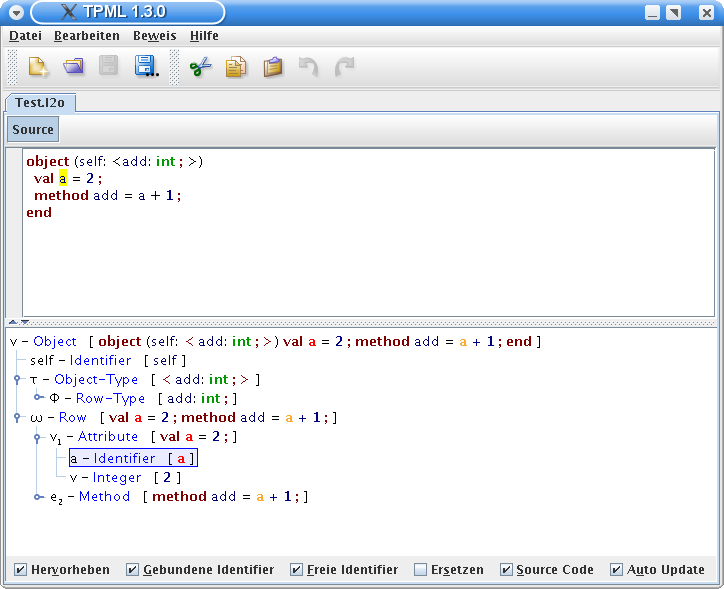
\includegraphics[height=14cm]{images/outline.png}
  \end{center}
}